\documentclass{article}
\usepackage[utf8]{inputenc}
\usepackage{amsthm, amssymb, mathtools, esdiff,stmaryrd, tcolorbox, bbm,float, physics}
\usepackage{tikz-cd}
\usepackage[export]{adjustbox}
\usepackage{hyperref}

\title{Measure theory notes}
\author{jyl20 }
\date{February 2022}
\newtheorem{theorem}{Theorem}[section]
\theoremstyle{definition}
\newtheorem*{definition}{Definition}
\newtheorem*{corollary}{Corollary}
\newtheorem{lemma}{Lemma}[theorem]
\newtheorem*{proposition}{Proposition}
\newtheorem*{proofsketch}{Sketch of proof}
\newtheorem{problem}{Problem}[section]
\newtheorem*{solution}{Solution}
\newtheorem*{remark}{Remark}
\newtheorem*{example}{Example}
\setlength{\parindent}{0pt}
\DeclareMathOperator*{\argmax}{arg\,max}
\DeclareMathOperator*{\argmin}{arg\,min}
\newlength{\NOTskip} 
\def\NOT#1{\settowidth{\NOTskip}{\ensuremath{#1}}%
	\hspace{0.5\NOTskip}\mathclap{\not}\hspace{-0.5\NOTskip}#1}
\renewcommand{\d}[1]{\ensuremath{\operatorname{d}\!{#1}}}
\newcommand*\interior[1]{\mathring{#1}}
\newcommand*\closure[1]{\overline{#1}}
\newcommand{\R}{\mathbb{R}}
\newcommand{\Rbar}{\overline{\R}}
\newcommand{\lsup}{\limsup_{n \to \infty}}
\newcommand{\linf}{\liminf_{n \to \infty}}
\newcommand{\ceq}{\coloneqq}
\newcommand{\limn}{\lim_{n\to \infty}}
\newcommand{\mn}{m\geq n}
\newcommand{\xseq}{(x_n)_{n \in \mathbb{N}}}
\newcommand{\setseq}{(A_n)_{n \in \mathbb{N}}}
\newcommand{\setunion}{\cup_{n \in \mathbb{N}}(A_n)}
\newcommand{\N}{\mathbb{N}}
\newcommand{\intm}[2][X]{\int_#1 #2 \, d \mu}
\newcommand{\sumlim}{\sum_{n=1}^\infty}
\newcommand{\measurablespace}{(\Omega, \mathcal{F})}
\newcommand{\measurespace}{(\Omega, \mathcal{F}, \mu)}
\newcommand{\F}{\mathcal{F}}
\newcommand{\C}{\mathcal{C}}
\newcommand{\G}{\mathcal{G}}
\newcommand{\B}{\mathcal{B}}
\newcommand{\I}{\mathcal{I}}
\newcommand{\Scal}{\mathcal{S}}
\newcommand{\Ccal}{\mathcal{C}}
\newcommand{\Lcal}{\mathcal{L}}
\newcommand{\A}{\mathcal{A}}
\newcommand{\Pbb}{\mathbb{P}}
\newcommand{\Pcal}{\mathcal{P}} 
\newcommand{\bracketsigma}{($\sigma$-)}
\newcommand{\probabilityspace}{(\Omega,\F,\Pbb)}
\newcommand{\1}{\mathbbm{1}}
\usepackage[left=1.5cm, right=1.5cm, top=1.5cm, bottom=1.5cm]{geometry}
\usepackage{multirow}
\usepackage{tabularx}
\usepackage[skip=1ex]{caption}

\begin{document}
\section{Comparison over different target distributions}
Different sampling methods, namely Metropolis-Hastings with a Gaussian random walk proposal (RW), MALA and ULA, are used to sample repeatedly from different target distributions. The target distributions are mixtures of Gaussians. For a certain point in time, the Wasserstein metric between the true distribution and the sampling distribution is approximated empirically by computing the Wasserstein metric between the uniform distribution over $k$ consecutive samples from the chain and $k$ independent samples from the target distribution. The above is repeated at various points in time to illustrate how the distance changes with time.
\\\\
Since each run is highly variable, the above is repeated for a number of independent runs to give a confidence interval for the estimated distance. On each run, the chain is initialised at a random point picked uniformly from $(-10, 0)$. The banded region shows the region which is within one standard deviation of the mean distance.
\\\\
To investigate the behaviour at different points in time, different plots are made for the burnin period (first 200 samples) and the 1000 samples after that. The choice of $k$, number of samples used to estimate the Wasserstein metric, is different for the burnin period and the next 1000 samples so the distances cannot be compared directly.

{\renewcommand{\arraystretch}{7}%
\begin{tabular}{|l|l|l|l|}
	\hline
	\multirow{2}{*}{Target pdf}
		&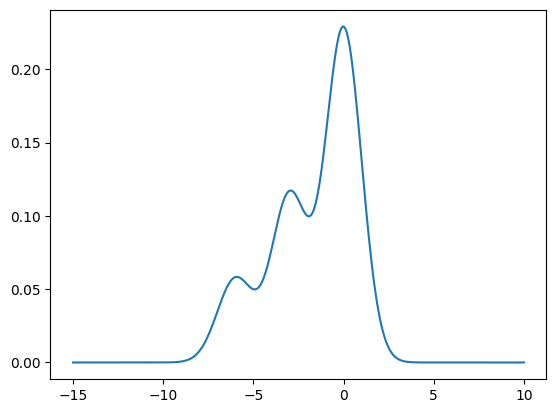
\includegraphics[width=.25\linewidth,valign=m]{targets/target1.png} 
	& 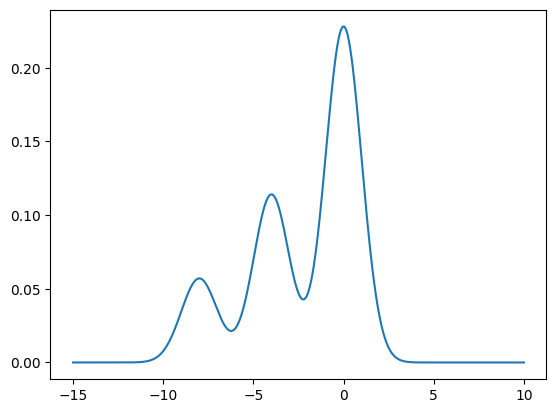
\includegraphics[width=.25\linewidth,valign=m]{targets/target2.png} & 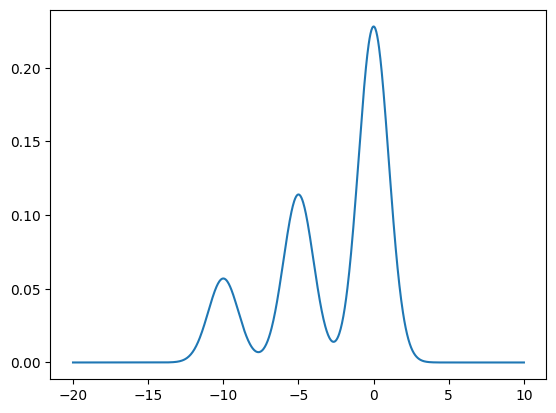
\includegraphics[width=.25\linewidth,valign=m]{targets/target3.png}\\
 & ${\scriptstyle \frac{1}{7} \mathcal{N}(-6, 1) + \frac{2}{7} \mathcal{N}(-3, 1) + \frac{4}{7}\mathcal{N}(0, 1)}$  & ${\scriptstyle \frac{1}{7} \mathcal{N}(-8, 1) + \frac{2}{7} \mathcal{N}(-4, 1) + \frac{4}{7}\mathcal{N}(0, 1)}$ & ${\scriptstyle \frac{1}{7} \mathcal{N}(-10, 1) + \frac{2}{7} \mathcal{N}(-5, 1) + \frac{4}{7}\mathcal{N}(0, 1)}$ \\
	\hline
	Burnin & 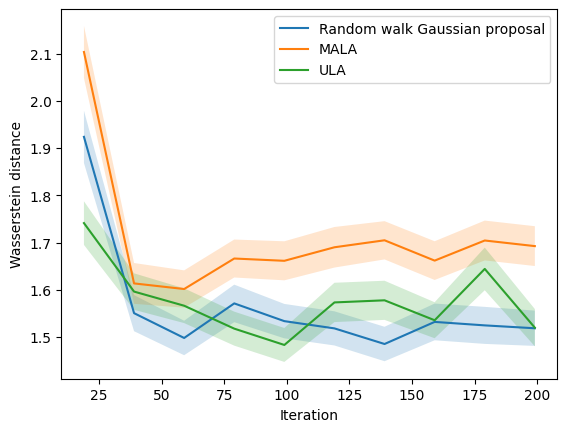
\includegraphics[width=.25\linewidth,valign=m]{Different targets/t11.png} & 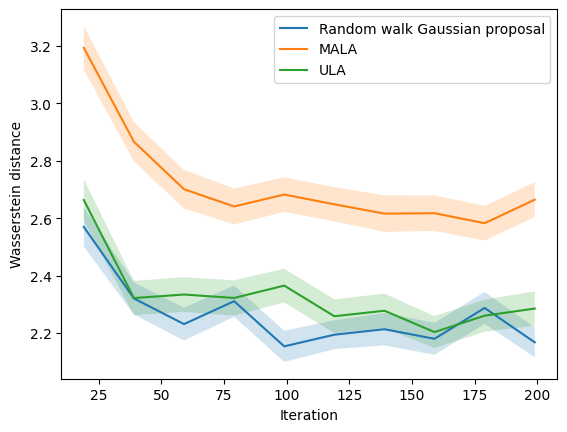
\includegraphics[width=.25\linewidth,valign=m]{Different targets/t21.png} & 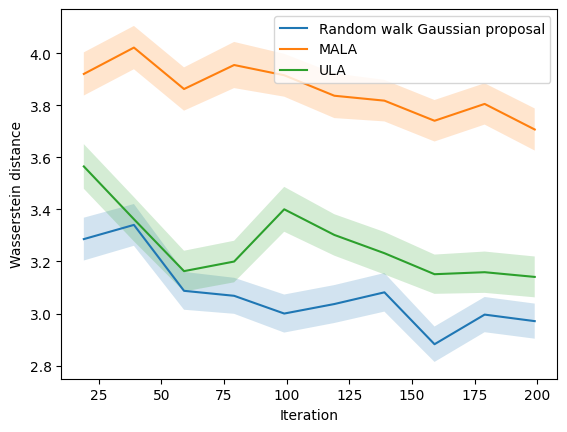
\includegraphics[width=.25\linewidth,valign=m]{Different targets/t31.png}\\
	\hline
	1000 samples & 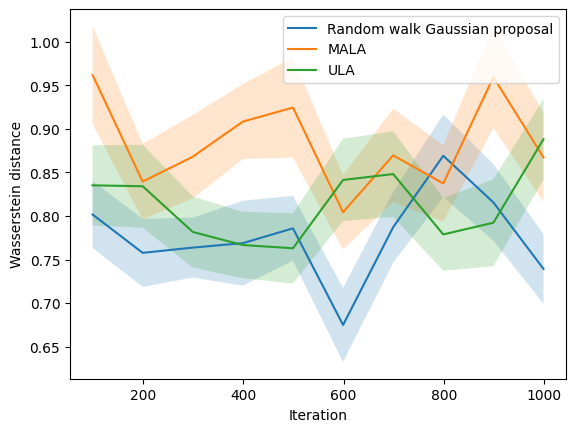
\includegraphics[width=.25\linewidth,valign=m]{Different targets/t12.png} & 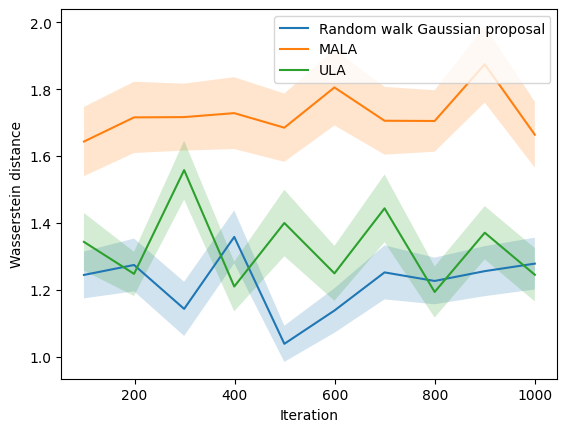
\includegraphics[width=.25\linewidth,valign=m]{Different targets/t22.png} & 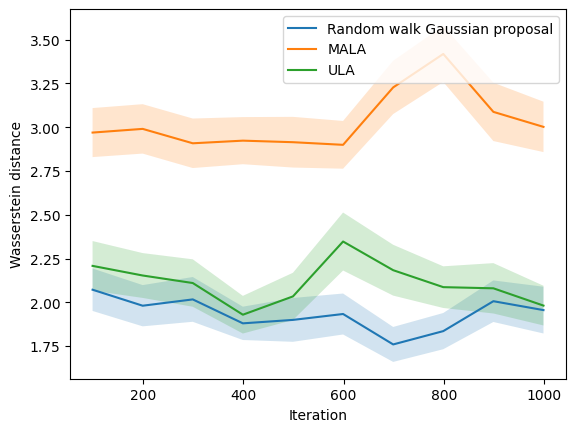
\includegraphics[width=.25\linewidth,valign=m]{Different targets/t32.png}\\
	\hline
\end{tabular}
}
\newpage
It seems that across the three targets, random walk performs the best, followed closely by ULA. MALA seems to perform substantially worse.
\\\\
This is a bit surprising because

\begin{itemize}
	\item MALA and ULA are similar in the sense that they are both gradient based
	
	\item MALA and RW are similar in the sense that they are metropolis-based
\end{itemize}
Maybe the difference is that MALA gets stuck at local maxima as shown later.
\\\\
TODO: 
\begin{enumerate}
	\item Check whether the method of computing empirical Wasserstein metric using consecutive samples from the same run actually make sense
\end{enumerate}


\newpage
\section{Trajectory of different sampling methods}
In this section, the trajectory of different sampling methods are compared. The target distribution is the rightmost target pdf from the previous section:
\[ 
 \frac{1}{7} \mathcal{N}(-10, 1) + \frac{2}{7} \mathcal{N}(-5, 1) + \frac{4}{7}\mathcal{N}(0, 1)
 \]
Trajectories of different sampling methods are plotted below. To ensure a fair comparison, all chains start at the mode of the leftmost peak (i.e. $x=-10$). 
\\\\
The plots are split into short run and long run, which aim to compare the non-asymptotic behaviour and the asymptotic behaviour respectively.
\\\\
For short runs, three independent chains are sampled for each method. For each chain, 3000 iterations are ran and the first 1000 are discarded.
\\\\
For long runs, one chain is sampled for each method and 11000 iterations are ran, the first 1000 of which are discarded.
{\renewcommand{\arraystretch}{4}%
\subsection{Short run}


	\begin{tabular}{|l|l|}
		\hline
		\multirow{3}{*}{RW} & \multicolumn{1}{l}{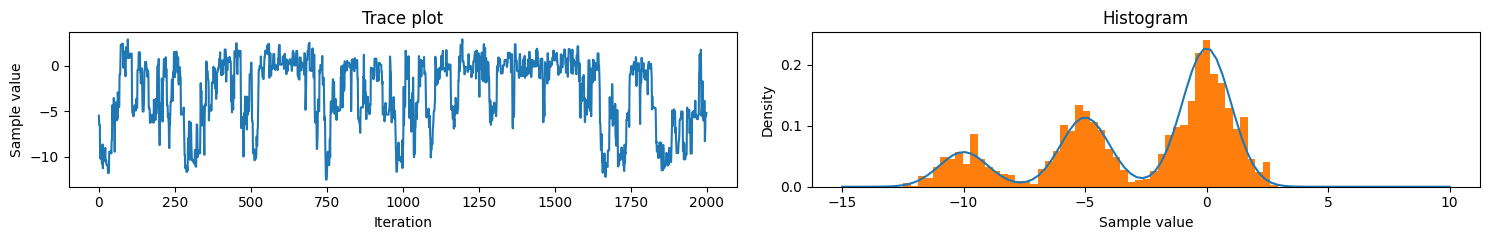
\includegraphics[width=0.8\linewidth, height=0.1\linewidth, valign=m]{diagnostics/rw1.png}} \\
							& \multicolumn{1}{l}{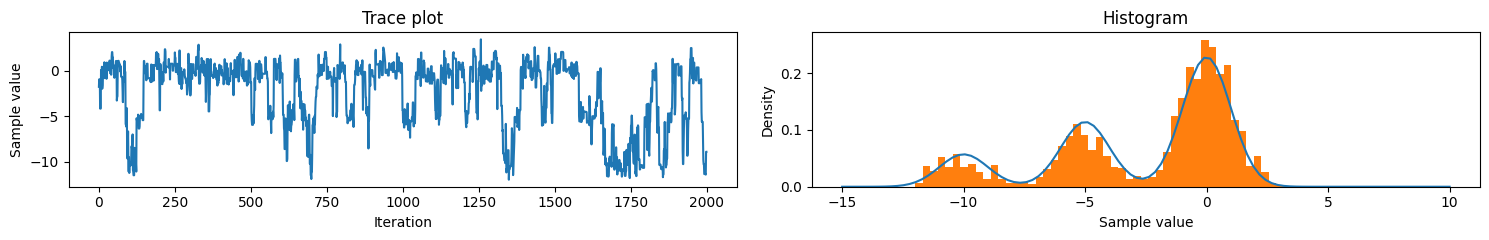
\includegraphics[width=0.8\linewidth, height=0.1\linewidth, valign=m]{diagnostics/rw2.png}} \\
							& \multicolumn{1}{l}{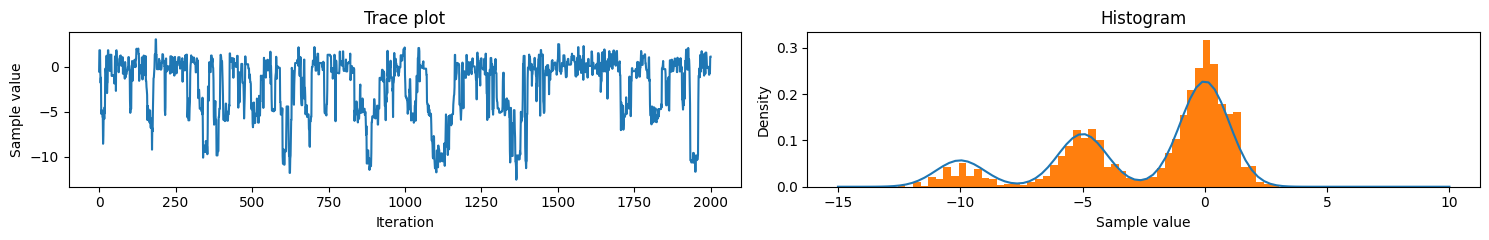
\includegraphics[width=0.8\linewidth, height=0.1\linewidth, valign=m]{diagnostics/rw3.png}} \\
		\hline
		
		\multirow{3}{*}{MALA} & \multicolumn{1}{l}{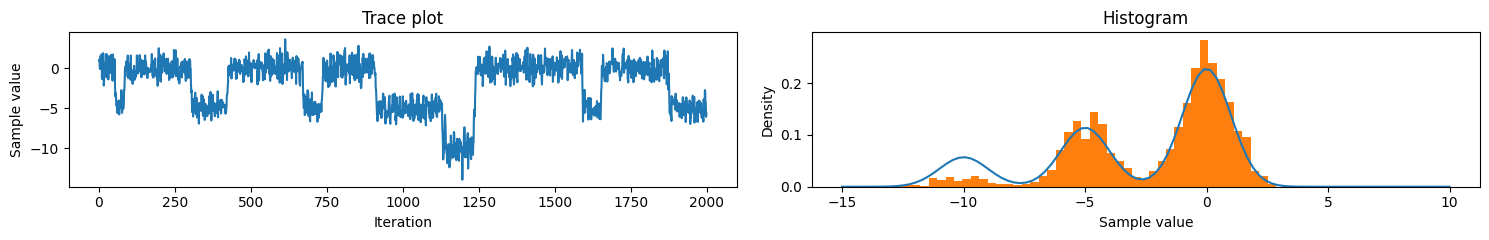
\includegraphics[width=0.8\linewidth, height=0.1\linewidth, valign=m]{diagnostics/mala1.png}} \\
& \multicolumn{1}{l}{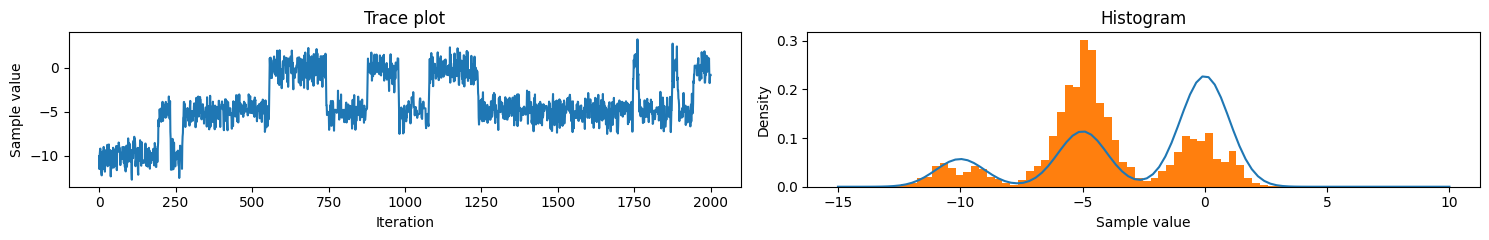
\includegraphics[width=0.8\linewidth, height=0.1\linewidth, valign=m]{diagnostics/mala2.png}} \\
& \multicolumn{1}{l}{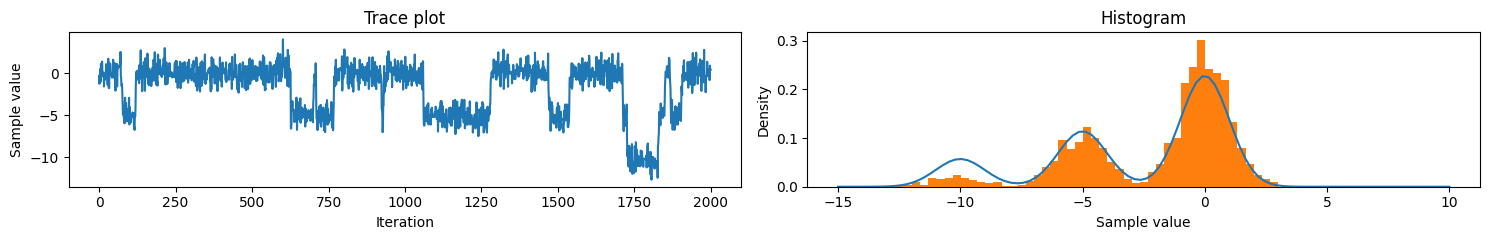
\includegraphics[width=0.8\linewidth, height=0.1\linewidth, valign=m]{diagnostics/mala3.png}} \\
\hline

		\multirow{3}{*}{ULA} & \multicolumn{1}{l}{\includegraphics[width=0.8\linewidth, height=0.1\linewidth, valign=m]{diagnostics/ULA1.png}} \\
& \multicolumn{1}{l}{\includegraphics[width=0.8\linewidth, height=0.1\linewidth, valign=m]{diagnostics/ULA2.png}} \\
& \multicolumn{1}{l}{\includegraphics[width=0.8\linewidth, height=0.1\linewidth, valign=m]{diagnostics/ULA3.png}} \\
\hline
	\end{tabular}
}

\subsubsection{Observations}
\begin{enumerate}
	\item MALA showed a bias towards local maxima of the pdf
	\item MALA shows long intervals of similar values on the trace plot
	\item MALA shows the greatest variation among different runs
	\item ULA showed a bias towards local minima of the pdf
\end{enumerate}
The first two observations are due to the gradient informed nature of MALA, which favours local maxima and makes it difficult to move from one maximum to another since it involves traversing a local minimum. The third observation is related to the above in the sense that the trajectory heavily depends on which peak the simulation gets stuck on.
\\\\
On the other hand, ULA has a bias towards local minima while MALA does not. The metropolis step in MALA rejects candidates which have a low probability under the target distribution and keeps the chain away from local minima. For ULA, no such correction is done so samples are relatively more likely to reach local minima.



{\renewcommand{\arraystretch}{5}%
\subsection{Long run}
\begin{tabular}{|l|l|}
	\hline
	RW & 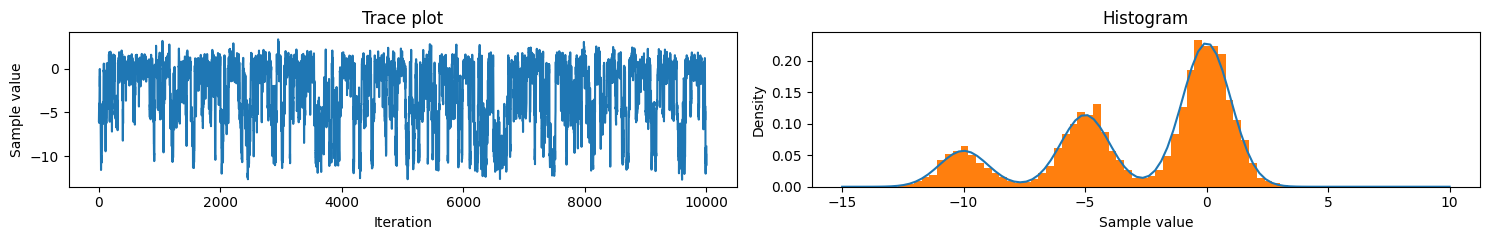
\includegraphics[width=0.8\linewidth,valign=m]{diagnostics/rwlong.png} \\
	\hline
	MALA & 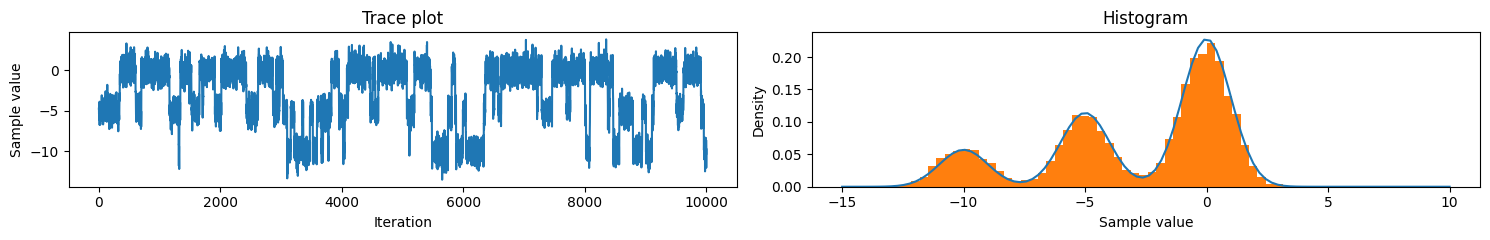
\includegraphics[width=0.8\linewidth,valign=m]{diagnostics/malalong.png} \\
	\hline
	ULA & 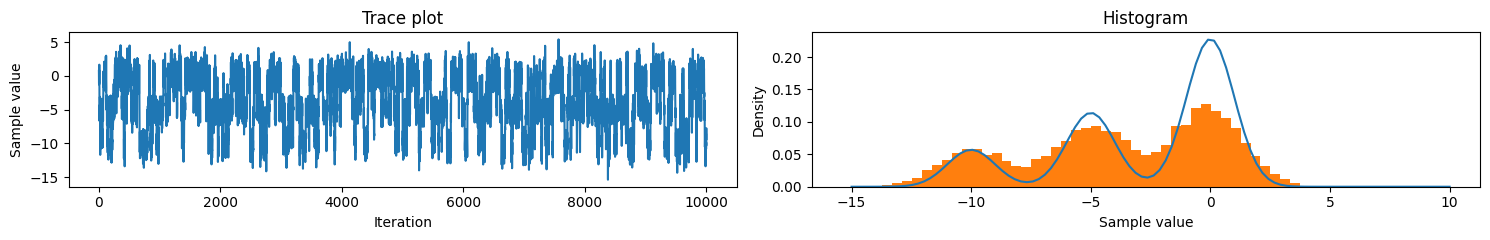
\includegraphics[width=0.8\linewidth,valign=m]{diagnostics/ulalong.png}\\
	\hline
\end{tabular}
}


\subsubsection{Observations}
Both Metropolis-based algorithms have empirical distributions which converge to the target pdf. ULA on the other hand does not converge to the target pdf, which is probably due to the discretisation error





\newpage
\section{Comparing different step sizes for ULA}
In the previous section, it is noted that the discretisation error may cause ULA to converge to a biased distribution. This section aims to investigate the impact of the step size on the behaviour of the ULA sampler.
\subsection{Wasserstein metric}
The Wasserstein metric for different step sizes / standard deviation is computed as before. \\
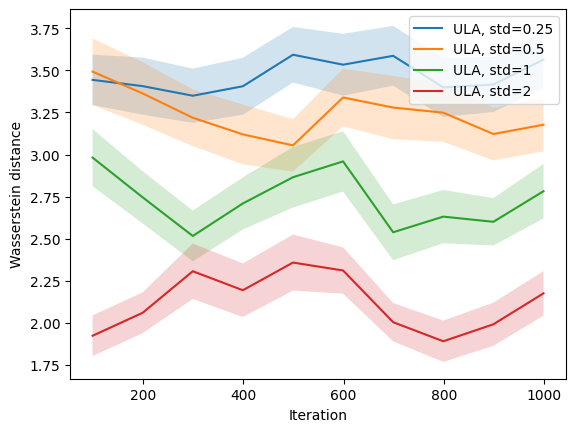
\includegraphics[width=0.8\linewidth,valign=m]{Different variance/var_plot.png}\\
\begin{remark}
	I am not sure what to make of this plot - it seems that the bigger the step size, the lower the distance. However, since the distance is computed using samples along the same chain, this might just be indicative of the fact that larger step sizes lead to samples which are less correlated along the same chain.
\end{remark}
\subsection{Trajectories for different step sizes}
\subsubsection{Short run}
{\renewcommand{\arraystretch}{4}%
	\begin{tabular}{|l|l|}
		\hline
	Step size & Plots\\

	\hline
	\multirow{3}{*}{2} & \multicolumn{1}{l}{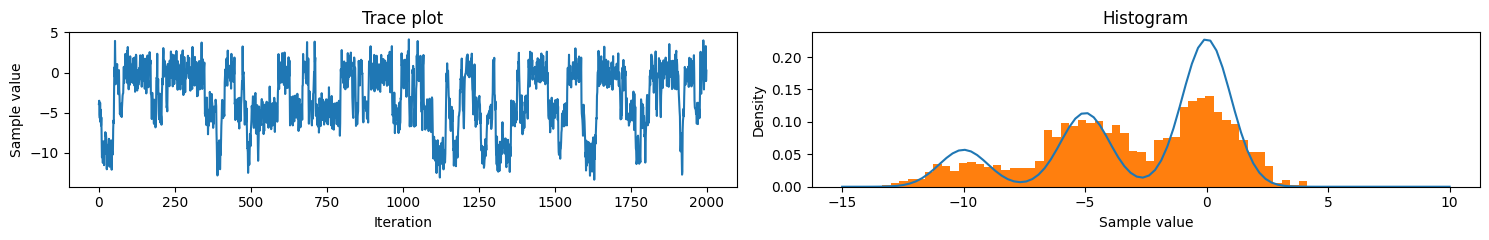
\includegraphics[width=0.8\linewidth, height=0.1\linewidth, valign=m]{Different variance/21.png}} \\
	& \multicolumn{1}{l}{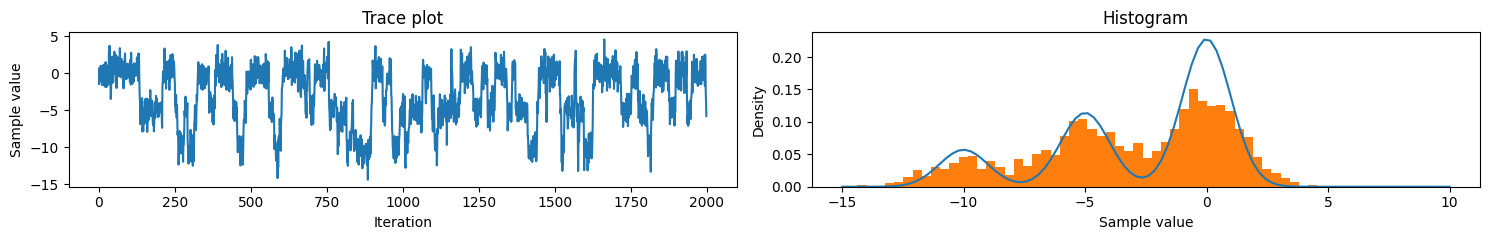
\includegraphics[width=0.8\linewidth, height=0.1\linewidth, valign=m]{Different variance/22.png}} \\
	& \multicolumn{1}{l}{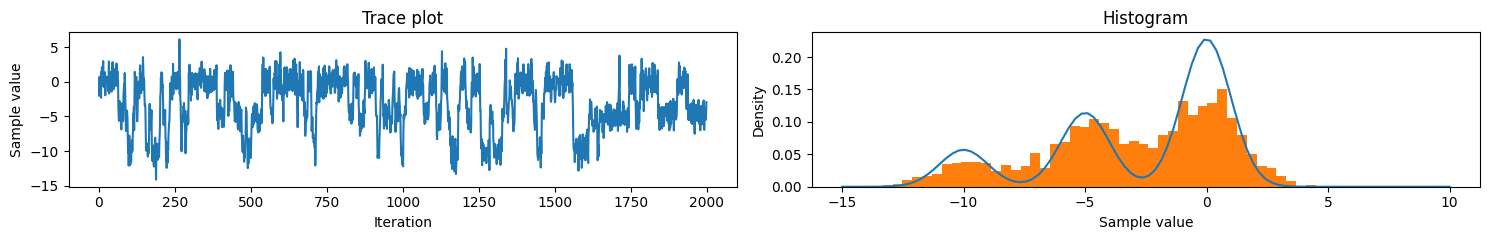
\includegraphics[width=0.8\linewidth, height=0.1\linewidth, valign=m]{Different variance/23.png}} \\
	\hline
	\multirow{3}{*}{1} & \multicolumn{1}{l}{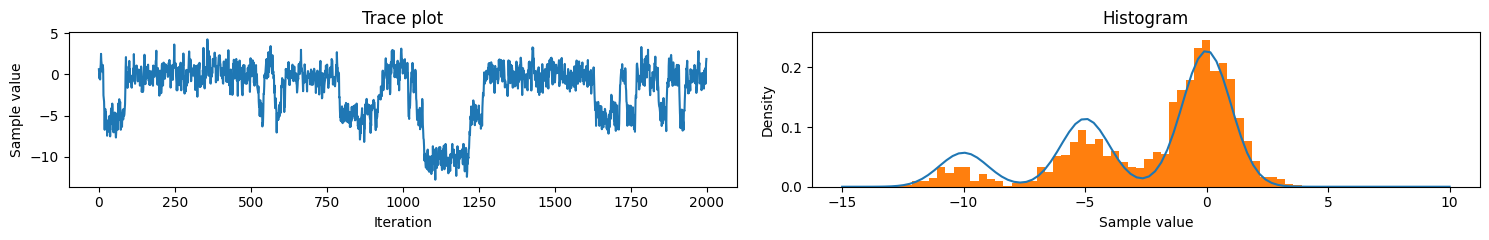
\includegraphics[width=0.8\linewidth, height=0.1\linewidth, valign=m]{Different variance/11.png}} \\
	& \multicolumn{1}{l}{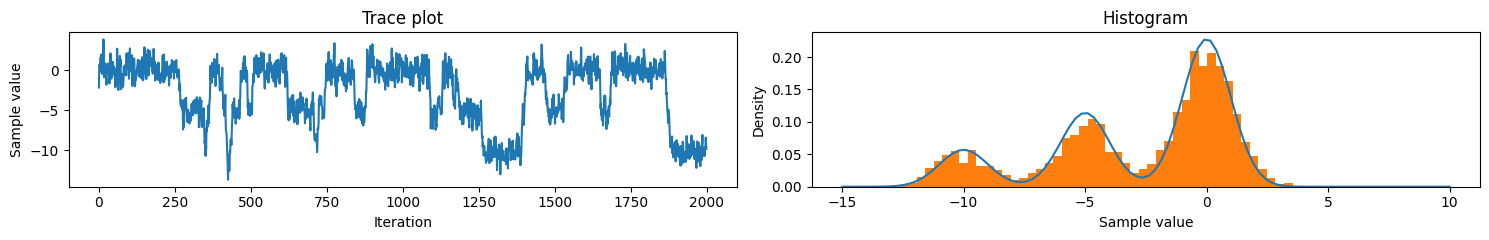
\includegraphics[width=0.8\linewidth, height=0.1\linewidth, valign=m]{Different variance/12.png}} \\
	& \multicolumn{1}{l}{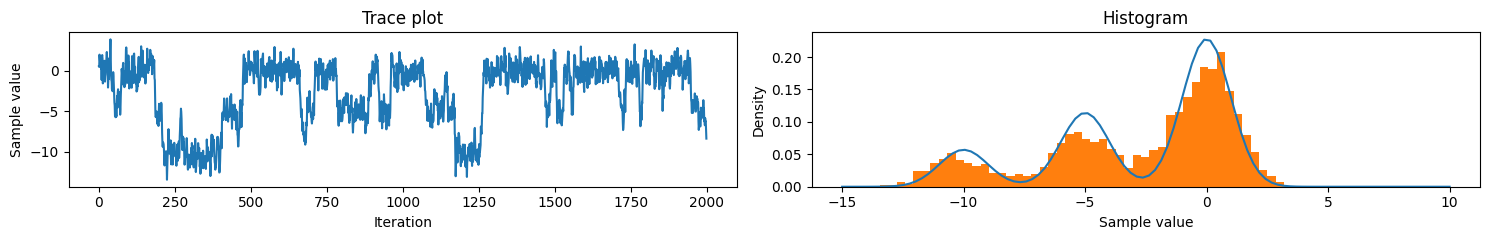
\includegraphics[width=0.8\linewidth, height=0.1\linewidth, valign=m]{Different variance/13.png}} \\
	\hline
	\multirow{3}{*}{0.5} & \multicolumn{1}{l}{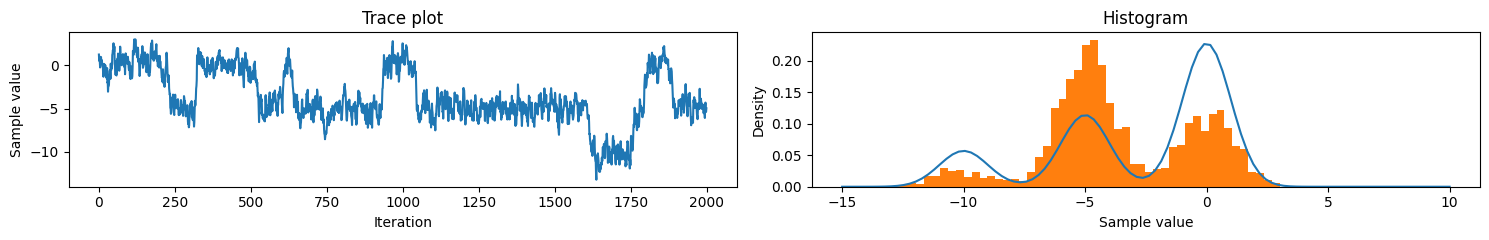
\includegraphics[width=0.8\linewidth, height=0.1\linewidth, valign=m]{Different variance/0_51.png}} \\
& \multicolumn{1}{l}{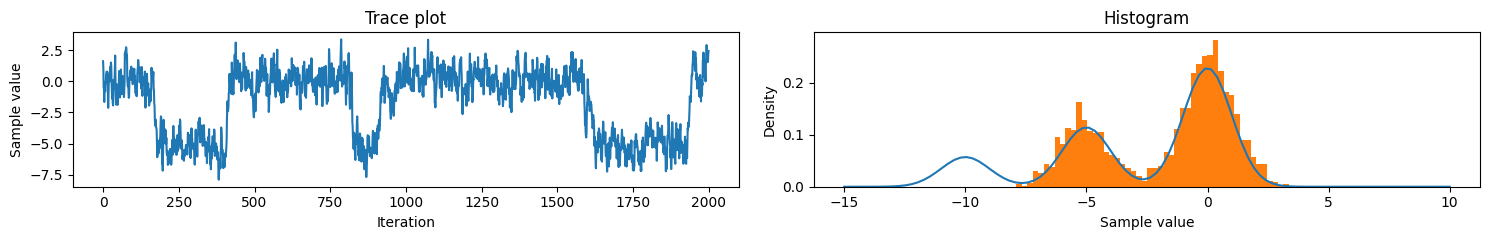
\includegraphics[width=0.8\linewidth, height=0.1\linewidth, valign=m]{Different variance/0_52.png}} \\
& \multicolumn{1}{l}{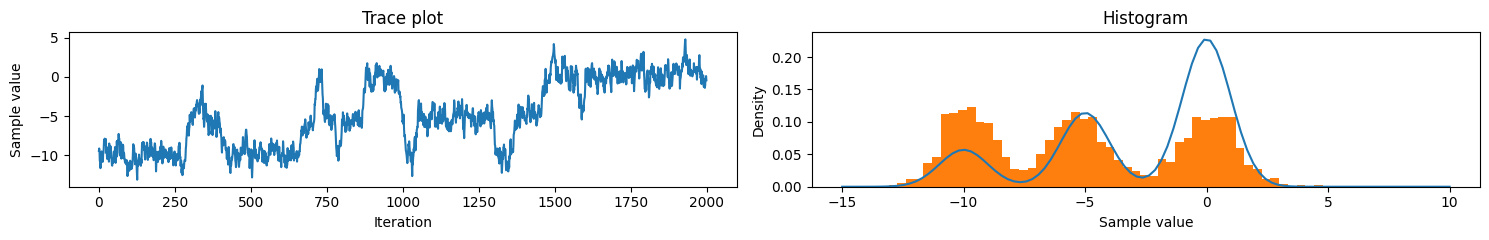
\includegraphics[width=0.8\linewidth, height=0.1\linewidth, valign=m]{Different variance/0_53.png}} \\
\hline
\end{tabular}

\begin{tabular}{|l|l|}
\hline
\multirow{3}{*}{0.25} & \multicolumn{1}{l}{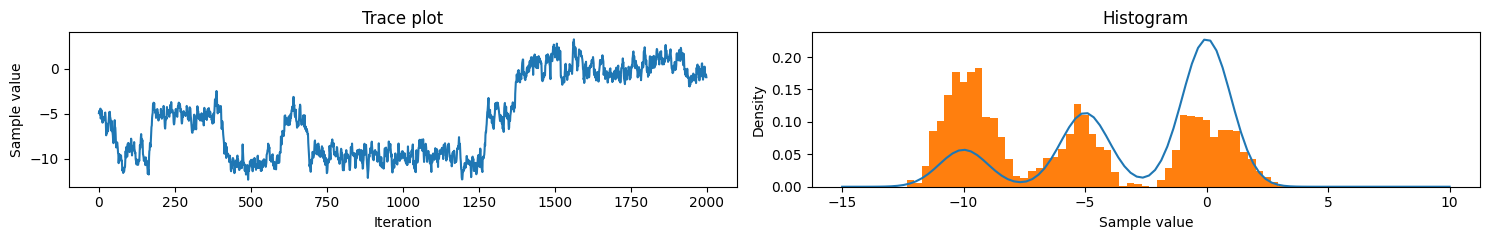
\includegraphics[width=0.8\linewidth, height=0.1\linewidth, valign=m]{Different variance/0_251.png}} \\
& \multicolumn{1}{l}{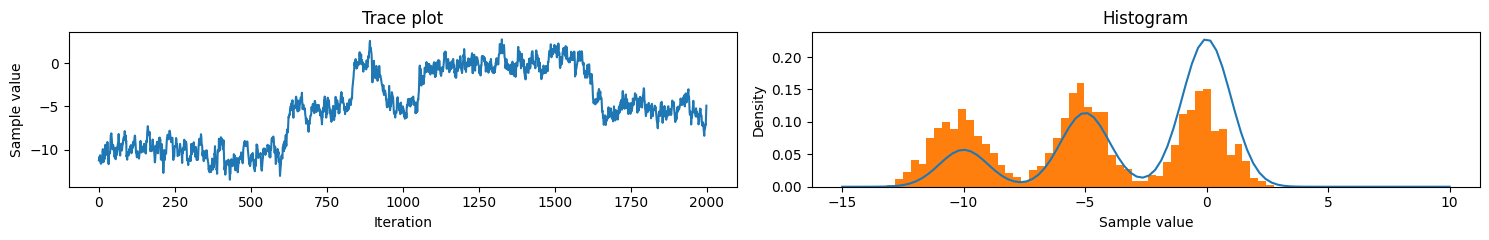
\includegraphics[width=0.8\linewidth, height=0.1\linewidth, valign=m]{Different variance/0_252.png}} \\
& \multicolumn{1}{l}{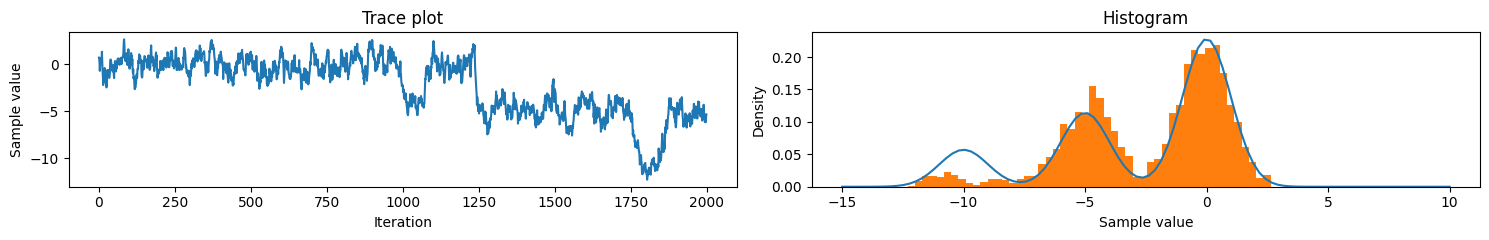
\includegraphics[width=0.8\linewidth, height=0.1\linewidth, valign=m]{Different variance/0_253.png}} \\
\hline
\end{tabular}
}

{\renewcommand{\arraystretch}{4}%
	\subsubsection{Long run}
	\begin{tabular}{|l|l|}
		\hline
		Step size & Plots\\
		\hline
		2 & 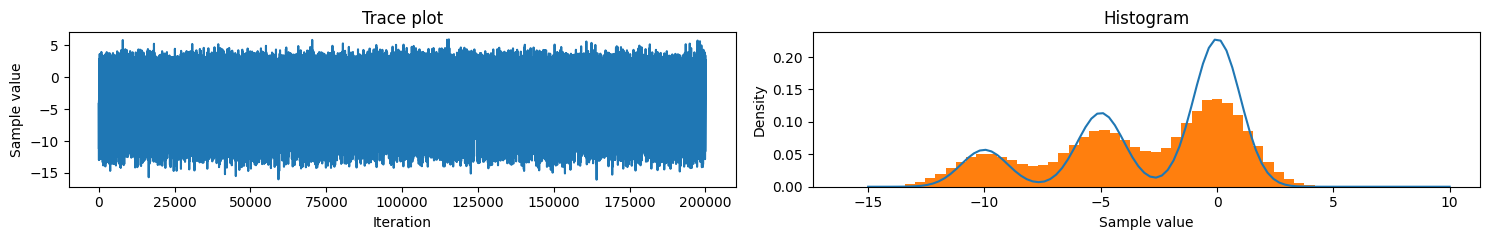
\includegraphics[width=0.8\linewidth, height=0.1\linewidth, valign=m]{Different variance/2long.png} \\
		\hline
1 & 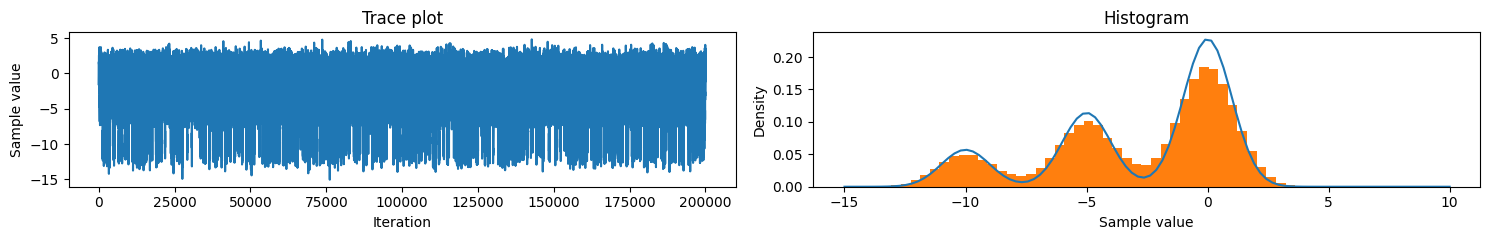
\includegraphics[width=0.8\linewidth, height=0.1\linewidth, valign=m]{Different variance/1long.png} \\
		\hline
0.5 & 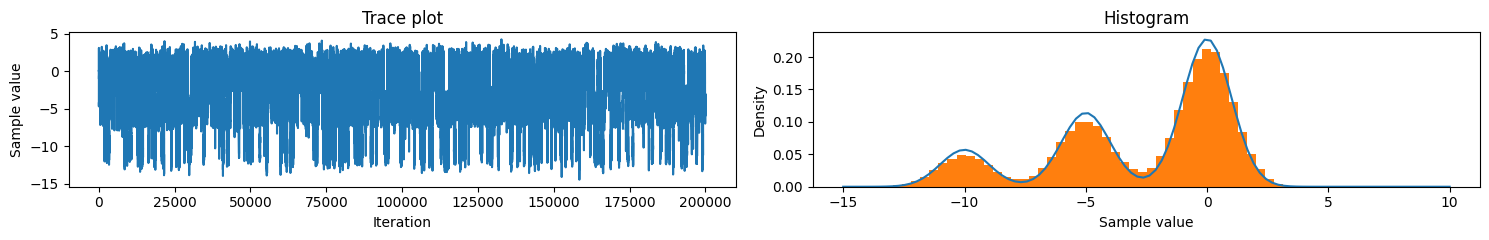
\includegraphics[width=0.8\linewidth, height=0.1\linewidth, valign=m]{Different variance/0_5long.png} \\
		\hline
0.25 & 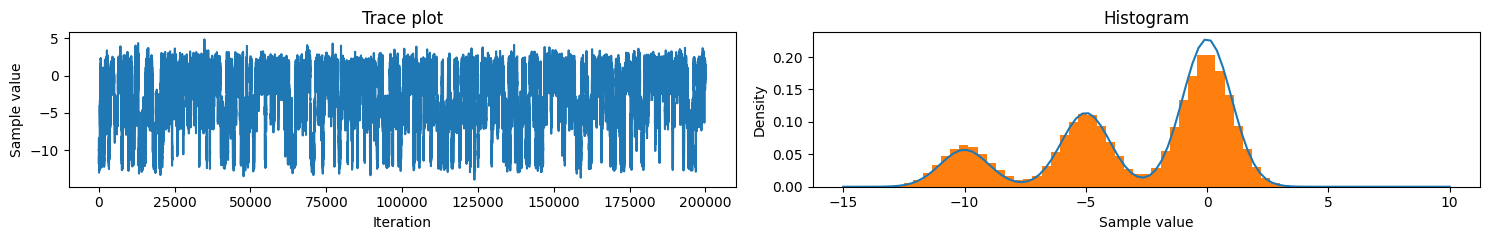
\includegraphics[width=0.8\linewidth, height=0.1\linewidth, valign=m]{Different variance/0_25long.png} \\
\hline
	\end{tabular}
}
\subsection{Observations}
From the short run plots, we see that as step size increases, the histogram becomes more similar across different runs. This may suggest that higher step size leads to faster convergence to the asymptotic sampling distribution.
\\\\
From the long run plots, we see that as step size decreases, the histogram becomes more like the target distribution, which suggests the asymptotic sampling distribution converges to the target distribution as the step size decreases.

\section{Github}
\url{https://github.com/justinlau20/Sampling}

\end{document}
